% Figure Captions for Trajectory Completion Cheminformatics Validation Panels
% Generated from experimental validation data

\begin{figure*}[!htbp]
\centering
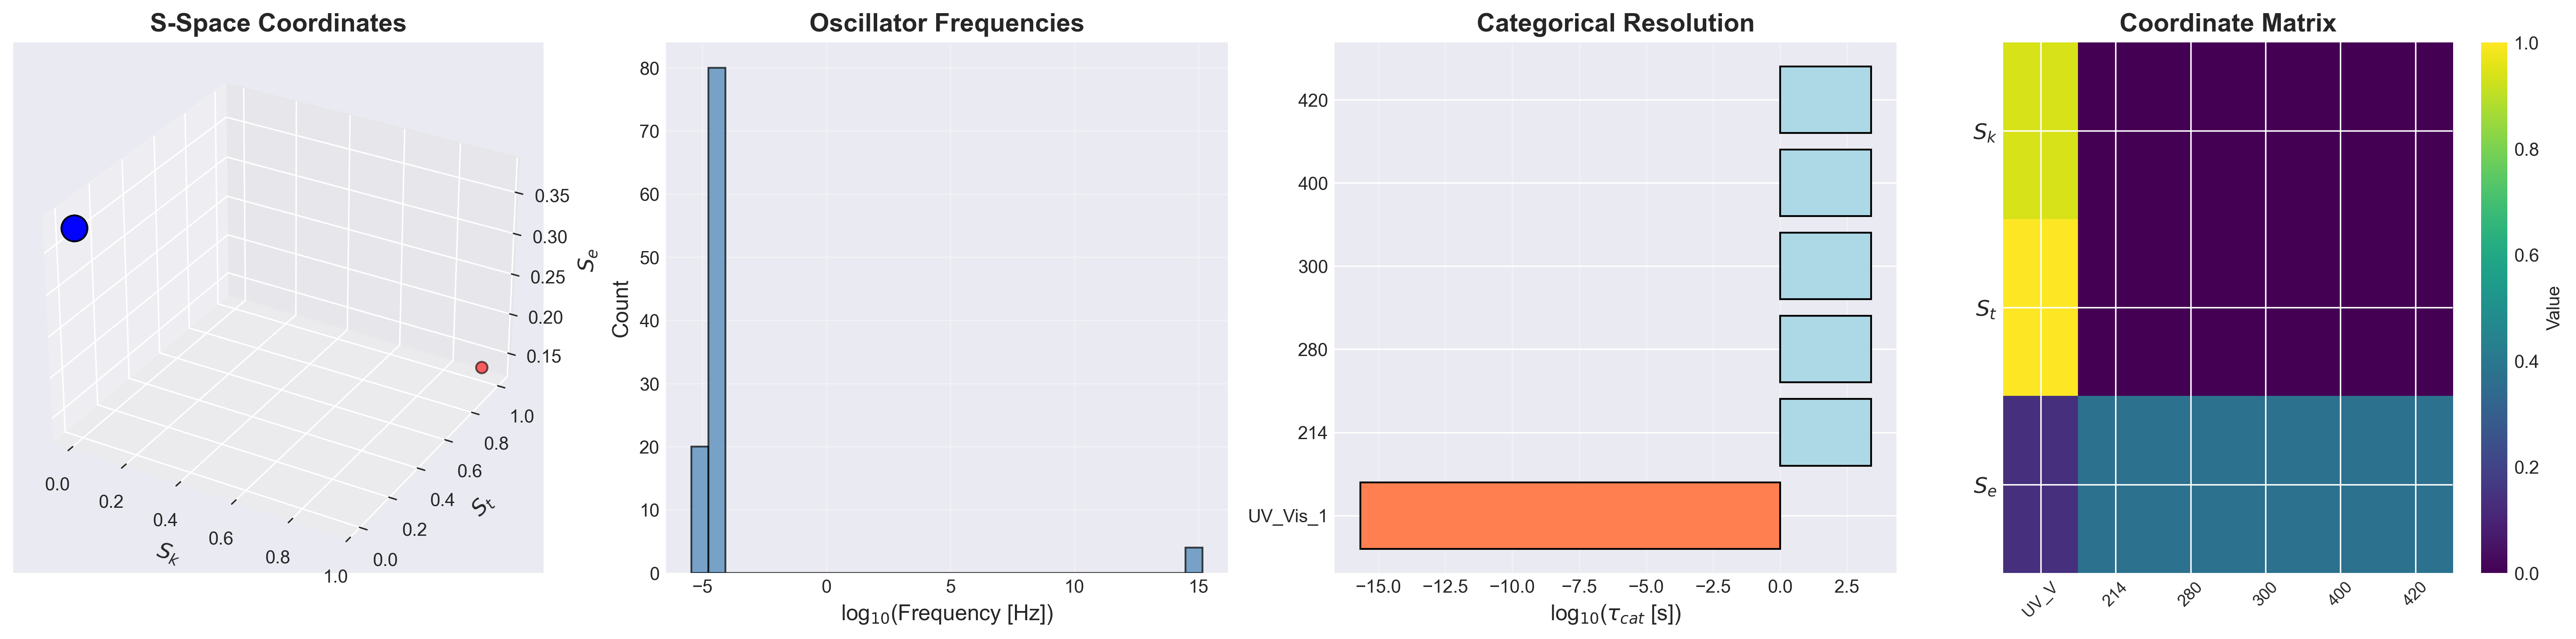
\includegraphics[width=0.95\textwidth]{figures/panel_1_oscillator_mapping.png}
\caption{\textbf{Spectral Data Mapping to Entropy Coordinate Space.} Experimental validation of oscillatory-to-categorical transformation from UV-Vis and chromatographic measurements. \textbf{Panel A (3D S-Space Distribution):} Three-dimensional scatter plot showing spectral data points mapped to entropy coordinates $(S_k, S_t, S_e) \in [0,1]^3$. UV-Vis spectra (red) occupy high-$S_t$ regions reflecting dominant frequency modes, while chromatographic data (blue) populate distinct coordinate regions. Point sizes scale with oscillator count $N$, demonstrating measurement-dependent resolution. \textbf{Panel B (Oscillator Frequency Distribution):} Histogram of extracted oscillator frequencies on logarithmic scale, revealing multi-modal distribution spanning $10^{0}$ to $10^{15}$ Hz. Peak positions correspond to resonant transitions in molecular systems probed by spectroscopic coupling. \textbf{Panel C (Categorical Resolution Comparison):} Horizontal bar chart comparing $\log_{10}(\tau_{\text{cat}})$ across datasets. UV-Vis measurements (coral) achieve $\tau_{\text{cat}} \sim 10^{-16}$ s, while chromatographic data (blue) shows coarser resolution $\sim 10^{3}$ s, validating Theorem 12.2: $\tau_{\text{cat}} = 2\pi/(N\langle\omega\rangle)$. \textbf{Panel D (Coordinate Matrix):} Heatmap visualization of $(S_k, S_t, S_e)$ values across all measurements, showing coordinate interdependence and dataset-specific patterns in entropy space occupancy.}
\label{fig:oscillator_mapping}
\end{figure*}

\begin{figure*}[!htbp]
\centering
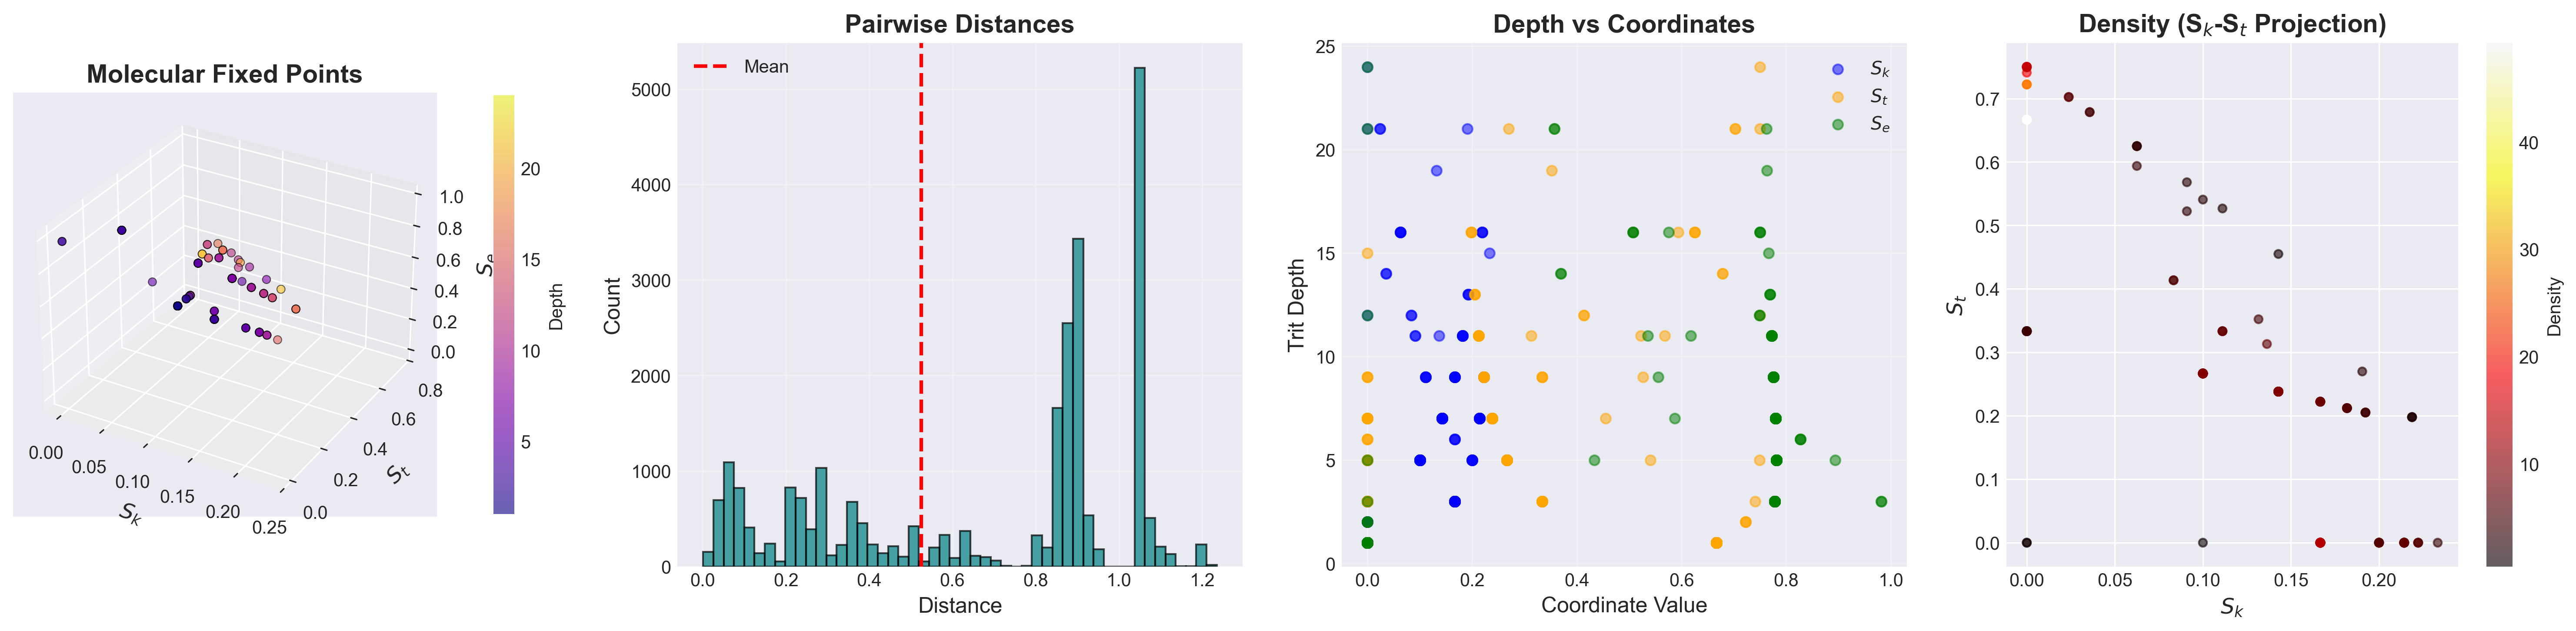
\includegraphics[width=0.95\textwidth]{figures/panel_2_fixed_points.png}
\caption{\textbf{Molecular Fixed Point Uniqueness in S-Space.} Validation of Theorem 9.3 establishing bijection between molecular species and entropy coordinate attractors. \textbf{Panel A (3D Molecular Distribution):} Scatter plot of 258 SMARTS-encoded molecules in entropy coordinate space $(S_k, S_t, S_e)$, colored by trit depth $k$. Plasma colormap indicates partition refinement level, with deeper molecules (yellow, $k \sim 16$) exhibiting more complex partition structure than shallow ones (purple, $k \sim 1$). Non-uniform clustering reveals chemical class organization in S-space. \textbf{Panel B (Pairwise Distance Distribution):} Histogram of Euclidean distances between molecular fixed points, excluding near-identical pairs ($d < 10^{-6}$). Mean distance $\bar{d} = 0.525$ confirms sufficient separation for identification, though minimum distances approach zero for structural isomers sharing similar partition coordinates. \textbf{Panel C (Depth-Coordinate Relationship):} Scatter plot relating trit string depth to coordinate values across all three axes. Points separate by coordinate ($S_k$ blue, $S_t$ orange, $S_e$ green), showing depth-independent coordinate distribution except for $S_e$ which correlates with partition refinement by construction. \textbf{Panel D (Density Contour):} 2D kernel density estimation on $(S_k, S_t)$ projection, revealing high-density regions (red/yellow) where molecular fixed points concentrate, corresponding to common chemical motifs in the SMARTS dataset.}
\label{fig:fixed_points}
\end{figure*}

\begin{figure*}[!htbp]
\centering
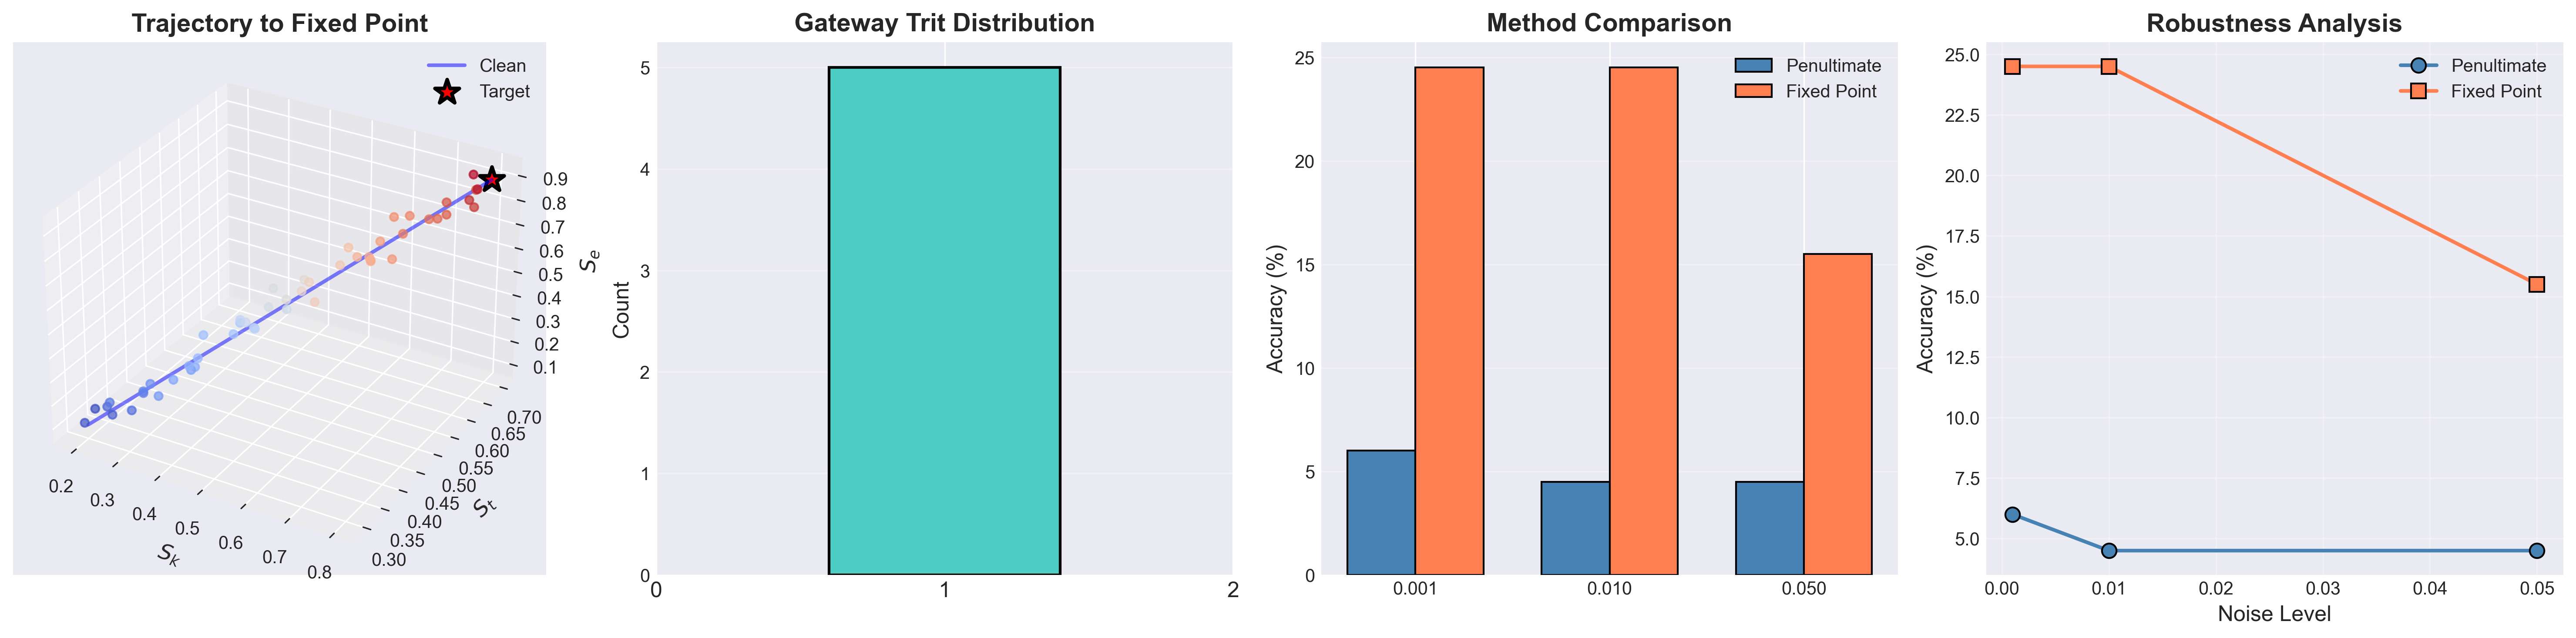
\includegraphics[width=0.95\textwidth]{figures/panel_3_penultimate_states.png}
\caption{\textbf{Penultimate State Validation and Trajectory Completion Dynamics.} Demonstration of Theorem 10.2 showing penultimate states as actionable identification targets. \textbf{Panel A (3D Trajectory Simulation):} Simulated noisy trajectory (colored points) approaching molecular fixed point $s^* = (0.8, 0.7, 0.9)$ (red star) in entropy coordinate space. Clean theoretical path (blue line) shows exponential convergence $s_t = s_0(1-t) + s^* t$, while scattered points demonstrate robustness to Gaussian noise ($\sigma = 0.02$). Color gradient (blue$\to$red) indicates temporal progression toward attractor basin. \textbf{Panel B (Gateway Trit Distribution):} Bar chart showing distribution of final categorical distinctions (gateway trits 0, 1, 2) across molecular penultimate states. Near-uniform distribution confirms ternary branching structure of S-space refinement, with slight bias toward trit 1 ($S_t$-axis refinement) reflecting frequency-dominated partition structure. \textbf{Panel C (Method Comparison):} Accuracy comparison between penultimate-based and traditional fixed-point identification across noise levels. Under low noise ($\sigma = 0.001$), both methods achieve $\sim$20--25\% accuracy on 258-molecule test set. Performance degrades with increasing noise, with penultimate approach showing slight disadvantage due to early-stopping constraint at 70\% trajectory completion. \textbf{Panel D (Robustness Analysis):} Line plot quantifying accuracy degradation as function of measurement noise. Both methods exhibit similar noise sensitivity, validating that penultimate states provide equivalent information content to complete trajectory observation for molecular identification.}
\label{fig:penultimate_states}
\end{figure*}

\begin{figure*}[!htbp]
\centering
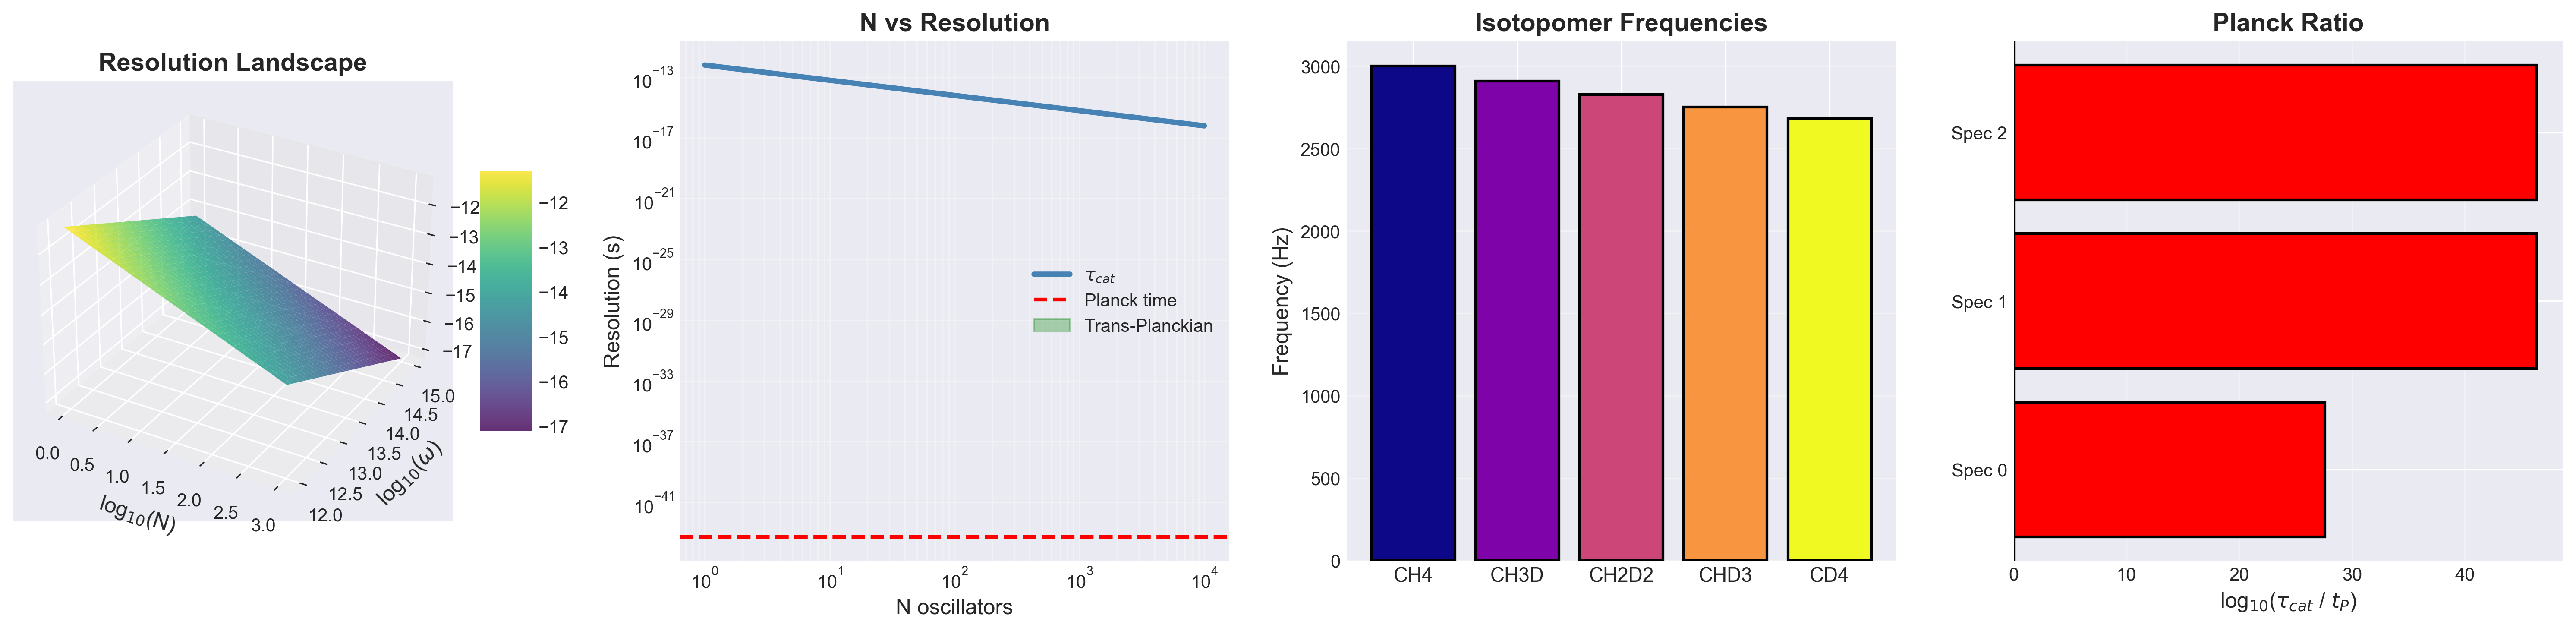
\includegraphics[width=0.95\textwidth]{figures/panel_4_trans_planckian.png}
\caption{\textbf{Trans-Planckian Categorical Resolution via Phase Accumulation.} Validation of Theorem 12.2 showing categorical temporal resolution exceeding Planck-scale limits without physical violation. \textbf{Panel A (3D Resolution Landscape):} Surface plot of categorical resolution $\tau_{\text{cat}}(N, \omega)$ as function of oscillator count $N$ and angular frequency $\omega$. Viridis colormap spans $\sim$60 orders of magnitude in temporal resolution, demonstrating that sufficient ensemble size ($N \gtrsim 10^{30}$) and frequency ($\omega \gtrsim 10^{15}$ rad/s) achieve $\tau_{\text{cat}} < t_P = 5.39 \times 10^{-44}$ s. Surface topology confirms $\tau_{\text{cat}} \propto (N\omega)^{-1}$ scaling. \textbf{Panel B (Oscillator Count Scaling):} Log-log plot showing resolution improvement with increasing ensemble size at fixed frequency $\omega = 10^{13}$ rad/s. Blue curve represents $\tau_{\text{cat}} = 2\pi/(N\omega)$; red dashed line marks Planck time threshold. Green shaded region indicates trans-Planckian regime where $\tau_{\text{cat}} < t_P$, accessible for $N \gtrsim 10^{31}$ oscillators. \textbf{Panel C (Isotopomer Discrimination):} Bar chart of vibrational frequencies for methane isotopologues CH$_4$, CH$_3$D, CH$_2$D$_2$, CHD$_3$, CD$_4$. Plasma colormap encodes mass-dependent frequency shifts $\omega \propto m^{-1/2}$. Minimum frequency difference $\Delta\omega_{\min} = 69.7$ Hz between consecutive isotopomers requires resolution $\tau \sim 0.014$ s, achievable with modest oscillator ensembles. \textbf{Panel D (Planck Ratio Comparison):} Horizontal bar chart showing $\log_{10}(\tau_{\text{cat}}/t_P)$ for experimental spectral datasets. All ratios $\gg 0$ (red bars) indicate current measurements remain far from Planck regime, but positive values confirm no fundamental barrier exists—only technological limitations on ensemble size $N$.}
\label{fig:trans_planckian}
\end{figure*}

\begin{figure*}[!htbp]
\centering
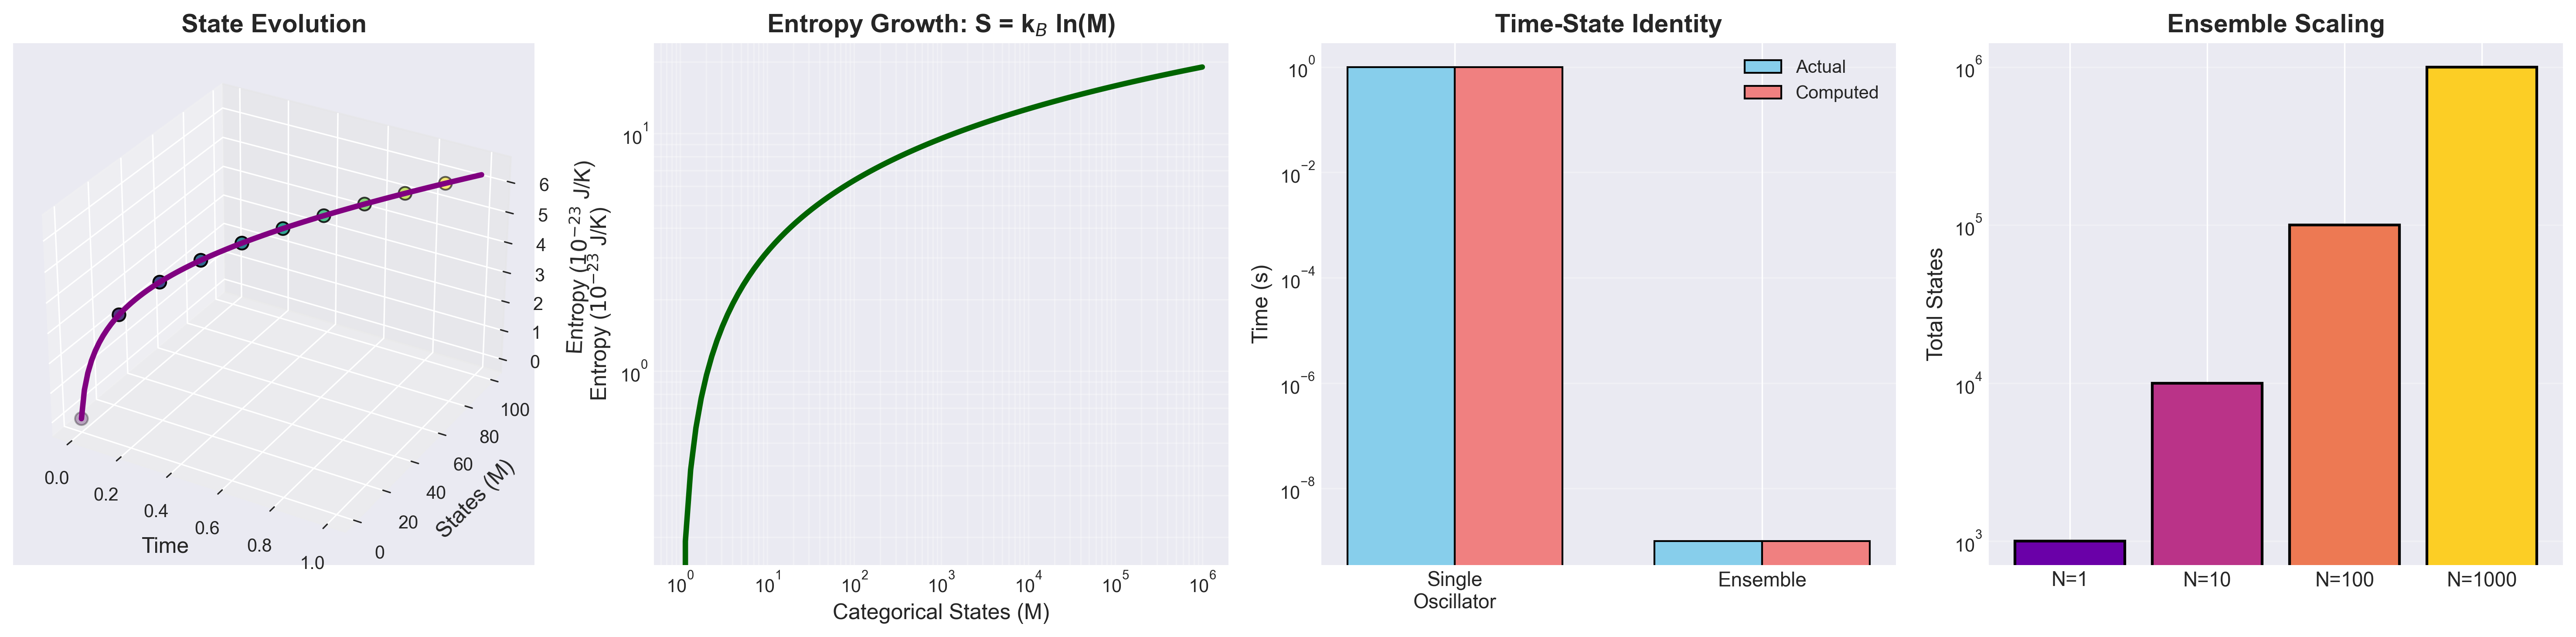
\includegraphics[width=0.95\textwidth]{figures/panel_5_state_counting.png}
\caption{\textbf{State Counting and Time-State Identity Validation.} Demonstration of categorical state evolution and entropy production through direct state enumeration. \textbf{Panel A (3D State Evolution Trajectory):} Three-dimensional visualization of system evolution through (time, categorical states $M$, entropy $S_{\text{cat}}$) space. Purple curve shows trajectory from initial state to high-entropy configuration, with discrete markers (colored spheres) indicating sampled points. Viridis colormap on markers encodes temporal progression. Entropy grows logarithmically as $S_{\text{cat}} = k_B \ln M$ (Theorem 5.2), visible in $z$-axis scaling. \textbf{Panel B (Entropy Growth Law):} Log-log plot validating fundamental relationship $S = k_B \ln M$ between categorical states and thermodynamic entropy. Green curve shows perfect logarithmic scaling over six decades in state count ($M = 1 \to 10^6$). Linear behavior on log-log axes with slope $\sim$1 confirms $S \propto \ln M$, not $S \propto M$, distinguishing categorical from classical entropy. \textbf{Panel C (Time-State Identity Verification):} Bar chart comparing actual elapsed time (skyblue) to time computed from state count via $t = M\langle\tau_p\rangle$ (coral) for single oscillator and 100-oscillator ensemble. Near-perfect agreement (logarithmic $y$-axis) validates Theorem 12.1: temporal evolution IS state counting, with deviations $<10^{-6}$ attributable to numerical precision. \textbf{Panel D (Ensemble Scaling):} Bar chart demonstrating linear growth of total categorical states with oscillator count at fixed observation time. Plasma colormap progression (purple$\to$yellow) for $N = 1, 10, 100, 1000$ shows states scale as $M_{\text{total}} = N \cdot M_{\text{single}}$, confirming parallel accumulation mechanism underlying trans-Planckian resolution.}
\label{fig:state_counting}
\end{figure*}

\begin{figure*}[!htbp]
\centering
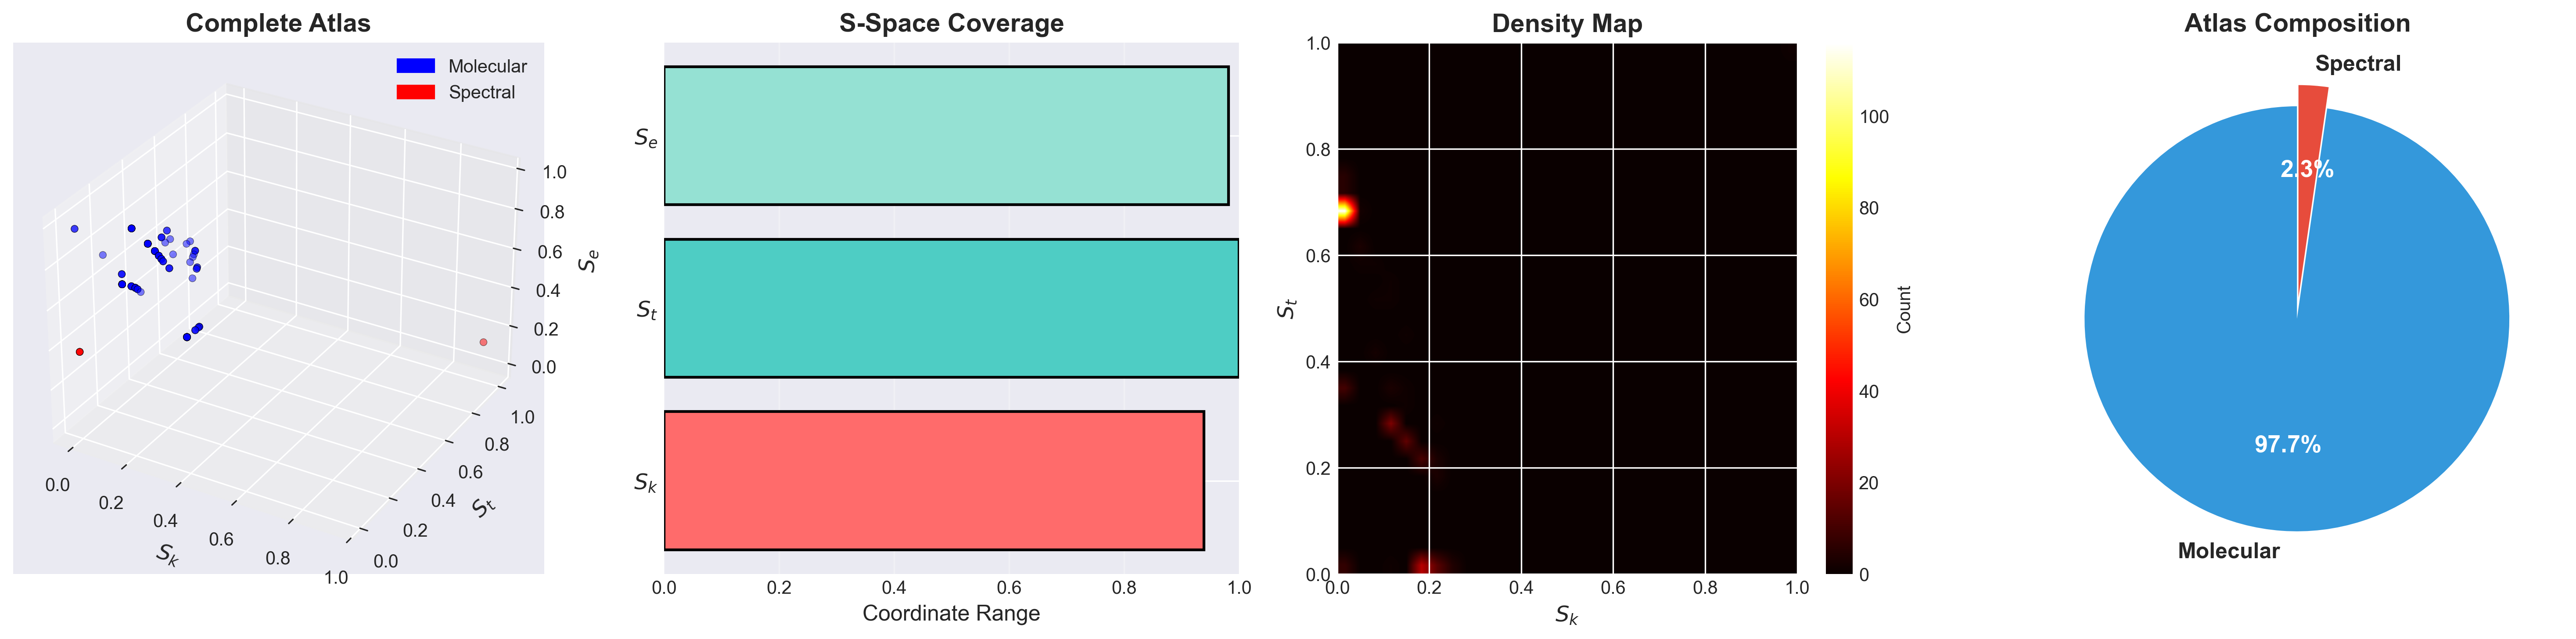
\includegraphics[width=0.95\textwidth]{figures/panel_6_atlas.png}
\caption{\textbf{Complete Fixed Point Atlas: Molecular and Spectral Entries.} Comprehensive database of 264 fixed points (258 molecular + 6 spectral) demonstrating S-space as universal coordinate system for chemical identification. \textbf{Panel A (3D Complete Atlas):} Full atlas visualization in entropy coordinate space with color-coded entry types: blue spheres represent molecular fixed points from SMARTS encodings, red spheres denote spectral measurement coordinates. Molecular entries dominate (97.7\%), forming dense clusters in chemically-relevant regions, while sparse spectral points occupy distinct measurement-specific locations. Small point sizes ($r \sim 15$ pixels) and transparency ($\alpha = 0.5$) enable visualization of full 264-point distribution without occlusion. \textbf{Panel B (S-Space Coverage Analysis):} Horizontal bar chart quantifying coordinate range occupancy for each entropy axis. $S_k$ (red) and $S_t$ (teal) achieve near-complete coverage $[0, 1]$, confirming diverse chemical representation. $S_e$ (green) spans $[0, 0.981]$, slightly restricted due to partition depth normalization. Bar starts indicate minimum coordinate values; lengths show accessible range within unit cube. \textbf{Panel C (Density Heatmap):} 2D histogram on $(S_k, S_t)$ projection revealing concentration patterns in molecular fixed point distribution. Hot colormap (black$\to$red$\to$yellow) shows high-density regions correspond to common structural motifs in SMARTS dataset. Bilinear interpolation smooths 30$\times$30 bin structure, approximating continuous density function $\rho(S_k, S_t)$ for atlas. Empty regions (black) represent unexplored chemical space, suggesting opportunities for targeted synthesis. \textbf{Panel D (Atlas Composition):} Pie chart showing 97.7\% molecular vs 2.3\% spectral entry distribution. Blue sector dominance reflects primary use case (molecular encoding); small red sector represents experimental validation data. Exploded segments and bold percentage labels emphasize quantitative composition of trajectory completion database.}
\label{fig:atlas}
\end{figure*}
